\documentclass[landscape]{tikzposter} %Options for format can be included here, for example portrait.

\usepackage{lutheme}
\usepackage{graphicx}
\graphicspath{{logo/}}

\usepackage[british]{babel}
% \usepackage{silence}
% \WarningFilter{latexfont}{Font shape}
% \WarningFilter{latexfont}{Some font}

%References
\usepackage{csquotes}
\usepackage[style=ieee]{biblatex}
\addbibresource{refs.bib}

 % Title, Author, Institute
\title{Template Poster}
\author{Author(s)}
\institute{Institute}

%Remove LaTeX tag at bottom of the poster
\tikzposterlatexaffectionproofoff

 %Choose Layout
\usetheme{LU}

\begin{document}

 % Title block with title, author, logo, etc.
\maketitle

%Input logos in relation to title node
%Go to the image bank https://lu-mediaportal.qbank.se for other images and logotypes.
\node[anchor=west, xshift=15mm] at (TP@title.west) {
\includegraphics[width=8cm]{lulogo.pdf}};
\node[anchor=east,xshift=-15mm] at (TP@title.east) {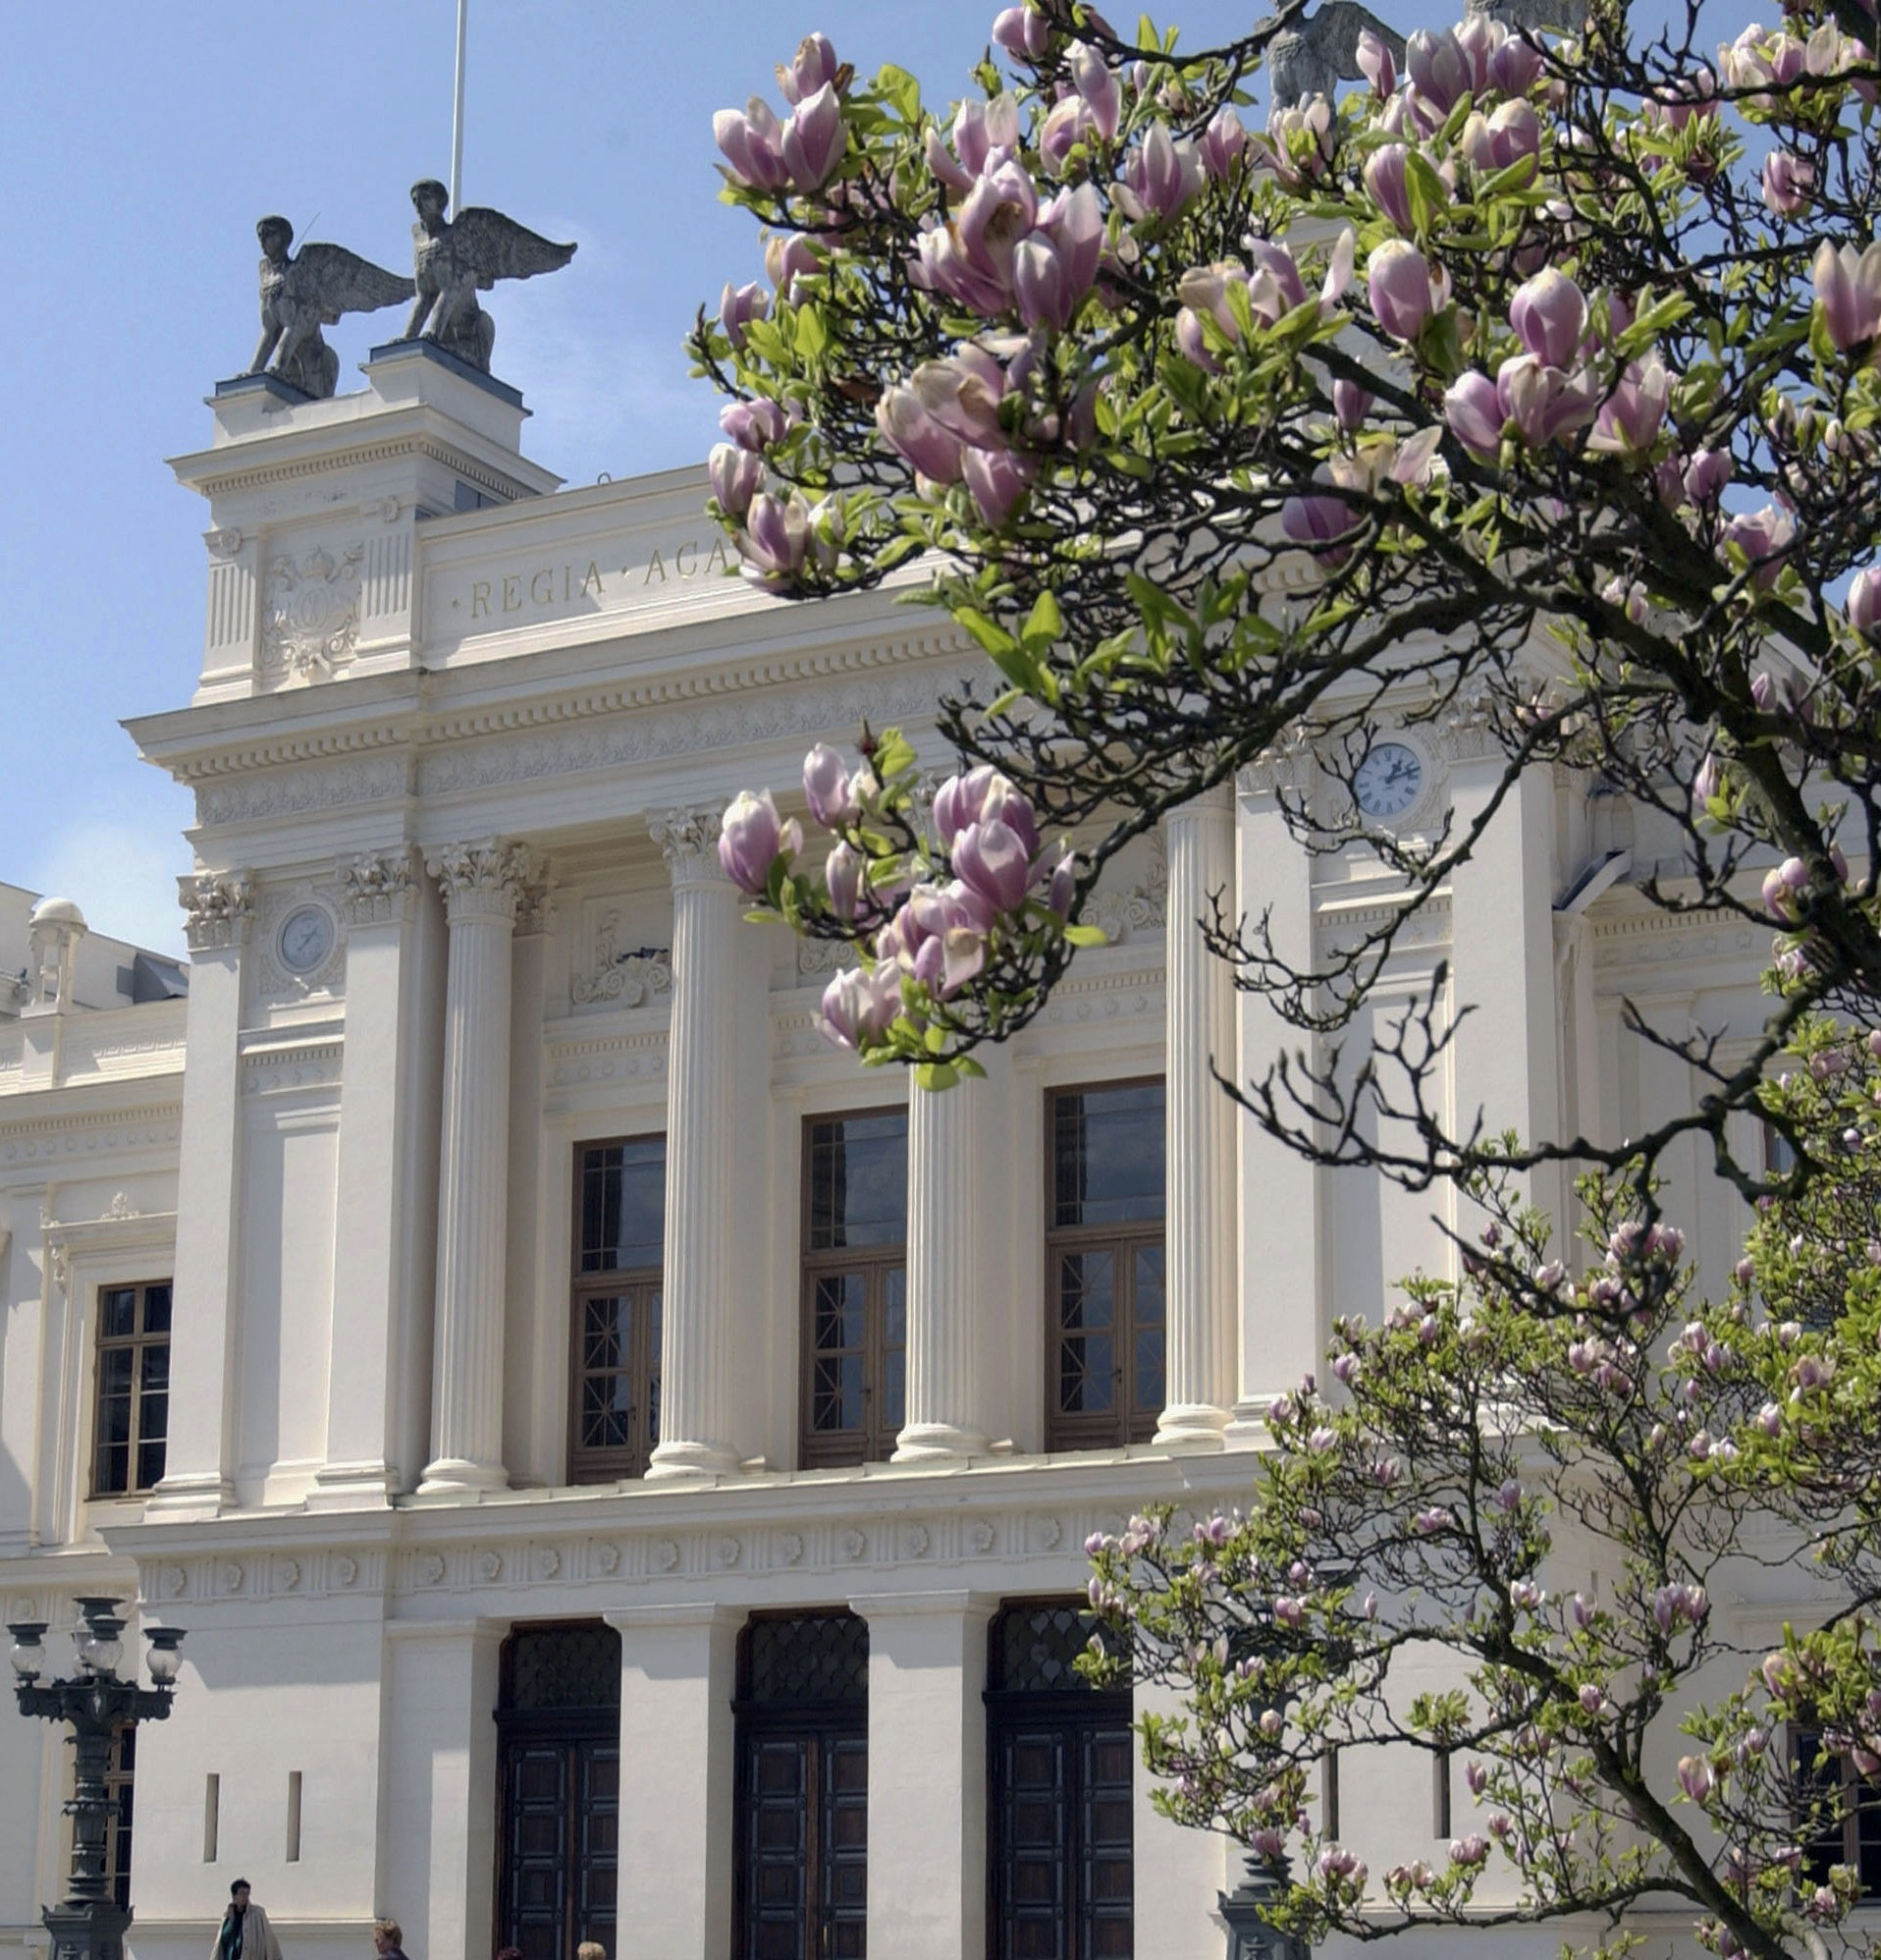
\includegraphics[width=10cm]{magnolia.jpg}};

 % First block
\block{Basic Block}{Text}
\begin{columns}

   % FIRST column
  \column{0.4}% Width set relative to text width

  \block{Large Column}{Text\\Text\\Text Text Text}
  \note{Note with default \\behavior}
  \note[targetoffsetx=12cm, targetoffsety=-1cm, angle=20, rotate=25]
  {Note \\ offset and rotated}

   % First column - second block
  \block{Block titles with enough text will automatically obey spacing requirements }
  {Text\\Text}

   % First column - third block
  \block[bodyfont=\sffamily]{Sample Block 4}{Block text till be {\rmfamily AGaramondPro-Regular}
  unless supplying the \texttt{bodyfont} argument.
  }

  \block{Table Block}{
    \begin{postertable}
      \centering
      \caption{This is some table text.}
      \begin{tabular}{|c|c|c|c|c|}
        \hline
        T & A & B & L & E\\
        \hline
      \end{tabular}
    \end{postertable}
  }

   % SECOND column
  \column{0.2}
   % Second column with first block's top edge aligned with with previous column's top.

   % Second column - first block
   % Need to reset font, pretty ugly
  \block[titleleft,bodyfont=\rmfamily]{Smaller Column}{Test}

   % Second column - second block
  \block[titlewidthscale=0.6, bodywidthscale=0.8]
  {Variable width title}{Block with smaller width.}

   % Second column - third block
  \block{}{Block with no title}

   % Second column - A collection of blocks in subcolumn environment.
  \begin{subcolumns}
    \subcolumn{0.27} \block{1}{First block.} \block{2}{Second block}
    \subcolumn{0.4} \block{Sub-columns}{Sample subblocks\\Second subcolumn}
    \subcolumn{0.33} \block{4}{Fourth} \block{}{Final Subcolumn block}
  \end{subcolumns}

   % Bottomblock
  \block{Final Block in column}{
    Sample block which might mention Einstein \cite{einstein}.
  }

  %THIRD column
  \column{0.4}
  \block{Figure Block}{
    \begin{posterfigure}
      \centering
      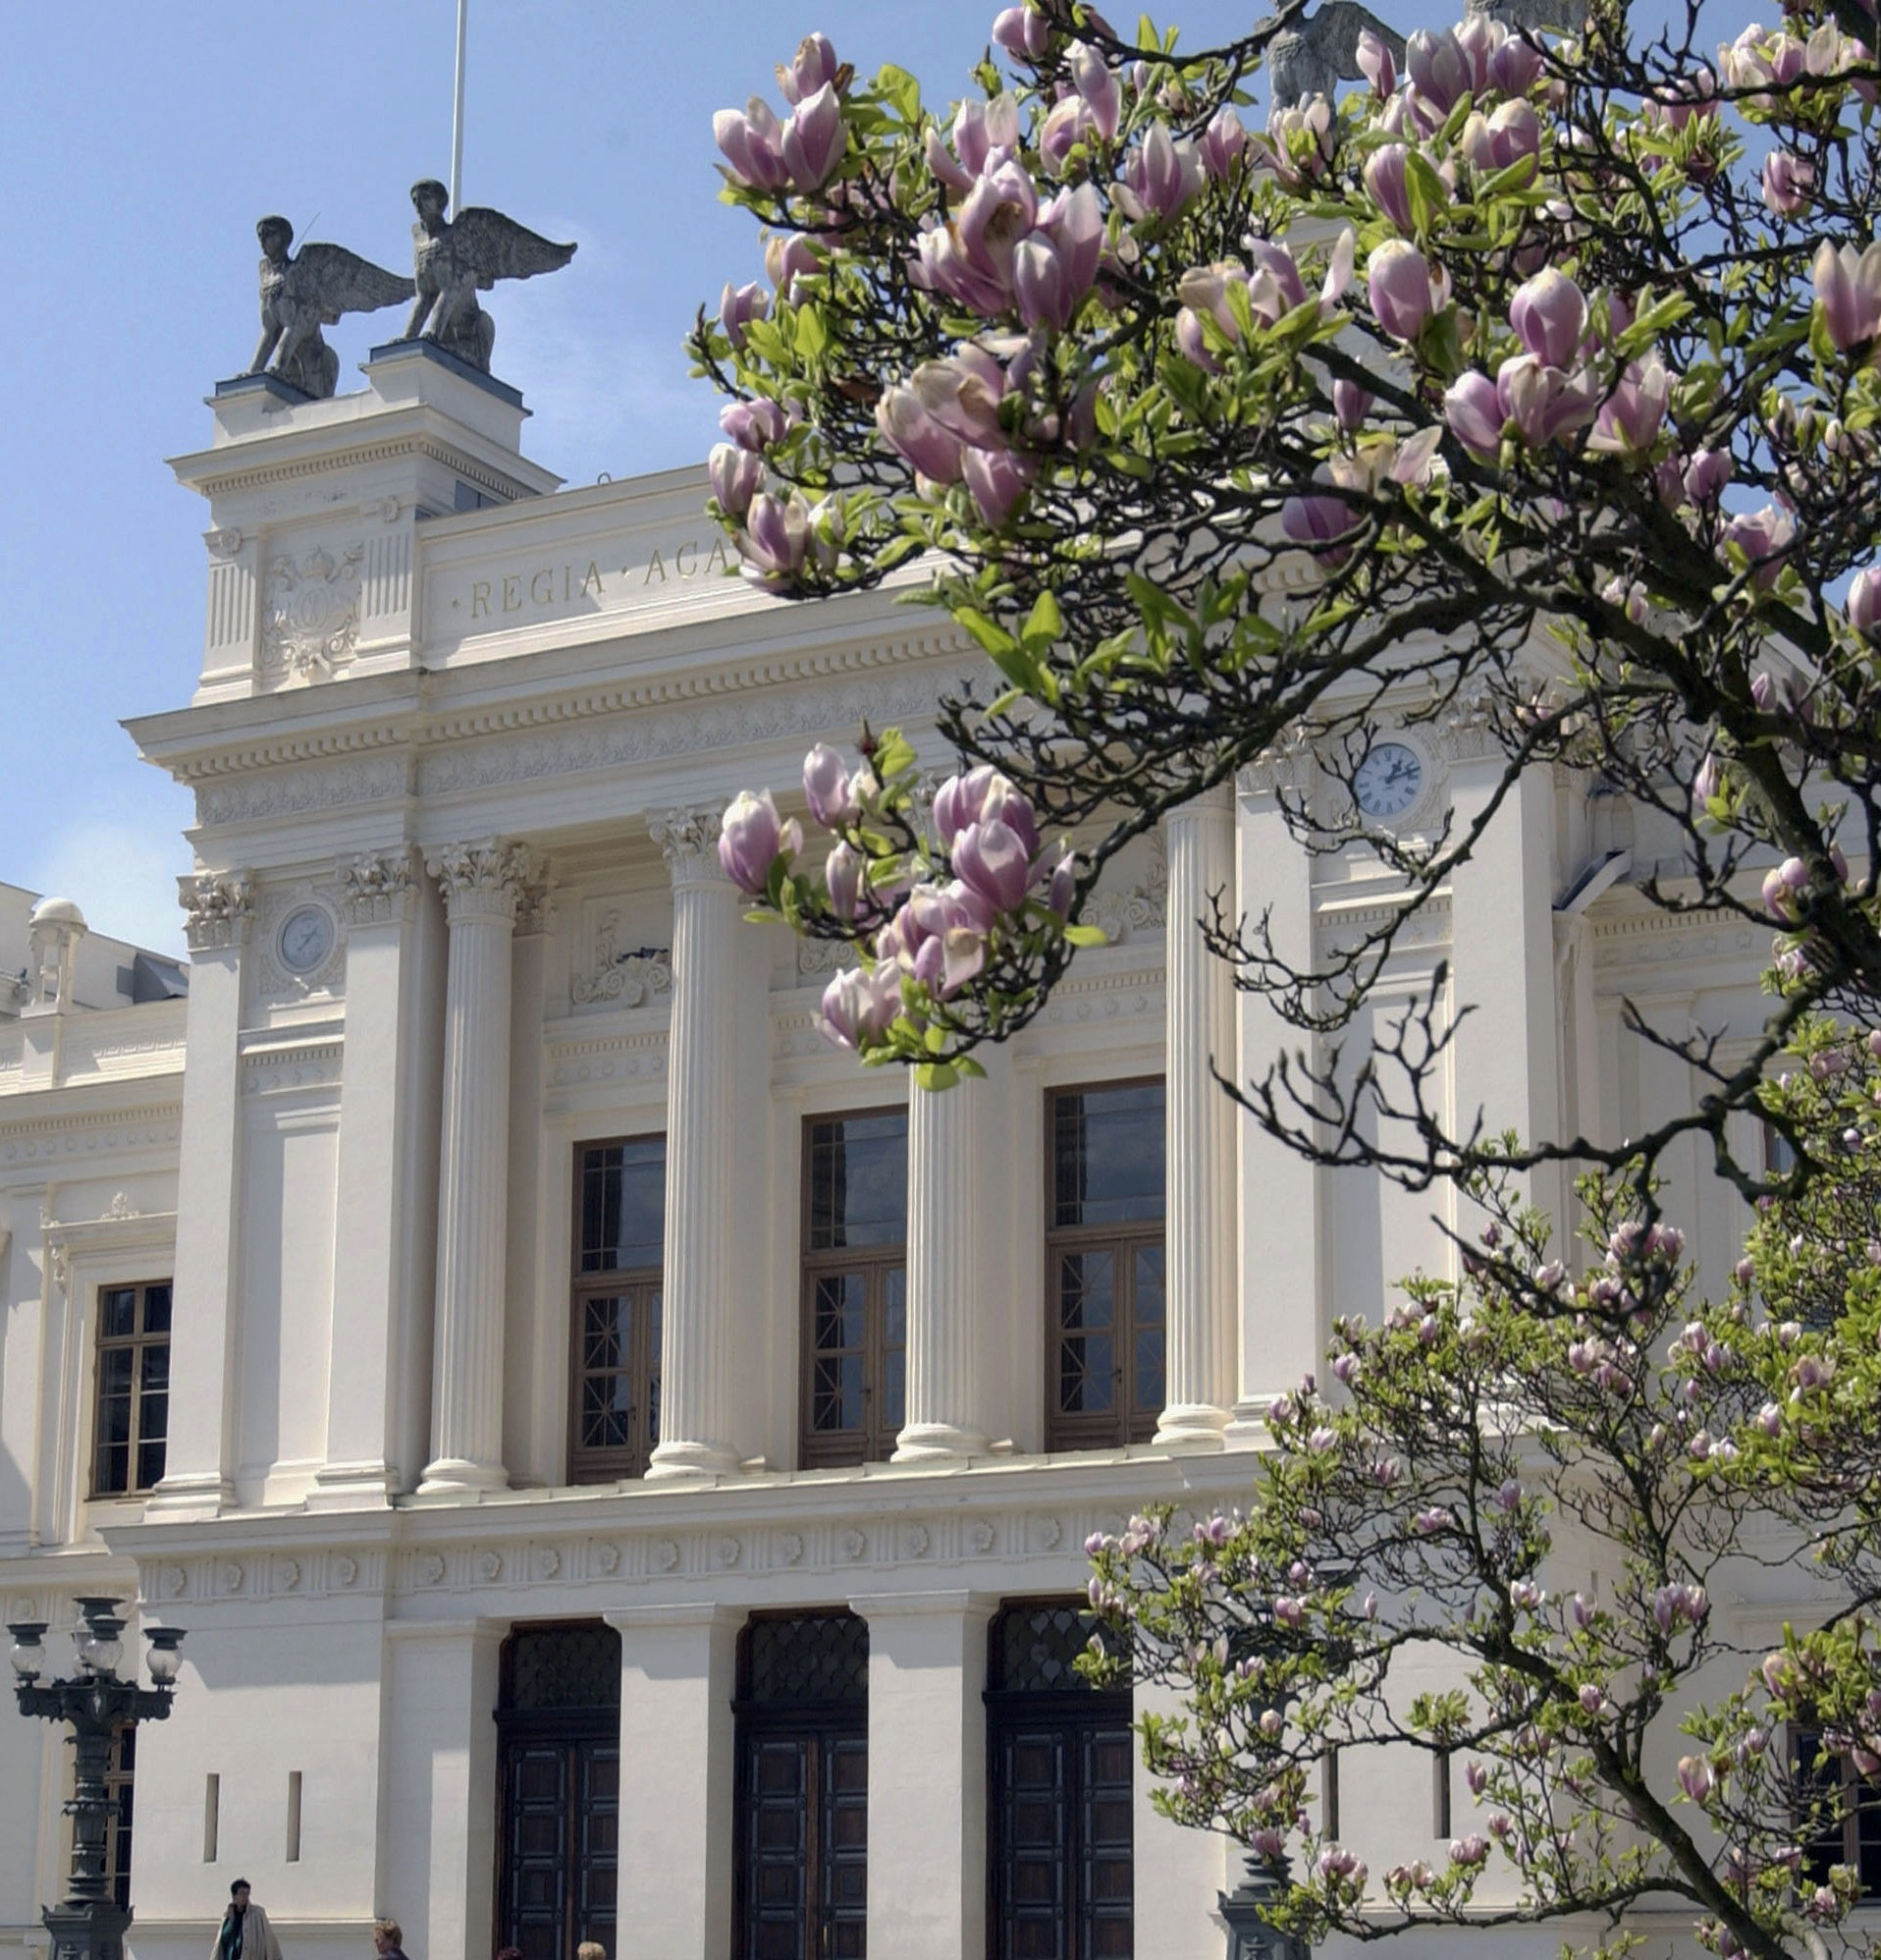
\includegraphics[width=0.6\textwidth]{magnolia}
      \caption{This is some figure text.}
    \end{posterfigure}
  }



  \block{Selected References}{
    \printbibliography[heading=none]
  }

\end{columns}

 % Final block
\block[titleleft, titleoffsetx=2em, titleoffsety=1em, bodyoffsetx=2em,%
 bodyoffsety=-2cm, roundedcorners=10, linewidth=0mm, titlewidthscale=0.7,%
 bodywidthscale=0.9, bodyverticalshift=2cm, titleright]
{Block outside of Columns}{Along with several options enabled}

\end{document}

\endinput
%%
%% End of file `tikzposter-template.tex'.
